\documentclass[10pt]{article}
\usepackage[utf8]{inputenc}
\usepackage[T1]{fontenc}
\usepackage{amsmath}
\usepackage{amsfonts}
\usepackage{amssymb}
\usepackage[version=4]{mhchem}
\usepackage{stmaryrd}
\usepackage[margin=0.5in]{geometry}
\usepackage{graphicx}
\begin{document}`

\noindent
(0,5 bodu) Rozhodněte, zdali je následující jazyk $L_1$ regulární, či nikoliv. Pokud jazyk není regulární, formálně toto tvrzení dokažte. Pokud jazyk regulární je, popište jej jedním z formalismů pro popis regulárních jazyků (tj. KA, RG, nebo RV). Dále pro něj nalezněte nejmenší  konstantu pumping lemma $p$ (jejíž existence je pro regulární jazyky v pumping lemma zaručena) a zdůvodněte, proč je vaše konstanta správná a nejmenší.

$$L_1=\left\{w: w \in\{\mathtt{a}, \mathtt{b}\}^{*} \wedge|w|_{\mathrm{a}} \bmod 3=|w|_{\mathrm{b}}\right\} \cap\left\{\mathtt{a}^{m} \mathtt{b}^{j} \mathtt{b}^{i}: m, j, i \in \mathbb{N}_{0} \wedge j<m\right\}$$

\noindent
Poznámka: Pomocí zápisu $|x|_a$ značíme počet symbolů $a$ v řetězci $x$.

\section*{Řešení:}

\begin{description}
\item[(1)]

Jazyk $L_1$ je průnikem dvou jazyků $L_{l}$ a $L_{r}$ ($l$ jako $left$, $r$ jako $right$), tj $L_1 = L_l \cap L_r$. Prozkoumame jednodtlive jazyky $L_l$ a $L_r$:

Jazyk $L_l$:

$$L_l = \left\{w: w \in\{\mathtt{a}, \mathtt{b}\}^{*} \wedge|w|_{\mathrm{a}} \bmod 3=|w|_{\mathrm{b}}\right\}$$

$L_l$ tedy reprezentuje všechny možné řetězce nad abecedou $\Sigma = \left\{a, b\right\}$, kde počet symbolu $b$ je roven počtu symbolů $a$ modulo 3. Důsledkem z toho je, že počet symbolů $b$ je minimalně $0$ a maximálně $2$. Příklady možných řetězců z tohoto jazyka:

$$L_l = \left\{
\epsilon,
ab, ba, aabb, abab, bbaa, baab, aaa, aaaab, aabaa, aaaaabb, aaaaaa, ... 
\right\}$$

Jazyk $L_r$:

$$L_r = \left\{\mathtt{a}^{m} \mathtt{b}^{j} \mathtt{b}^{i}: m, j, i \in \mathbb{N}_{0} \wedge j<m\right\}$$

Příklady řetězců:

$$L_r = \left\{
a, ab, abb, abbb, abbb...b, aab, aabb, aabb....b, aa...abb...b, ... 
\right\}$$

Všimneme si, že $L_r$ zadává určitou strukturu řetězce - všechny symboly $a$ se vyskytují pouze zleva, zprava pouze symboly $b$. 
Dále vidíme, že minimální řetězec je $w = a$, protože máme podmínku $j<m$, a zárověň víme že nejmenší možné $j$ je $0$ ($j\in\mathbb{N}_{0}$, tj. $m$ nemůže být $0$, (jinak bychom měli kontradicki, že $j$ musí být menší než nula a zárověň větší nebo rovnen nule). Tj. v podstatě platí, že $m \geq 1$, neboli $m \in \mathbb{N}$ ale bez nuly.

Další pozorování je, $i$ může být libovolné a nijak nezáleží na žádné jiné proměnné. Tj. $\forall m \in \mathbb{N}$, pokud zafixujeme $j = 0$, tak pomocí $i$ vygenerujeme libovolný počet symolů $b$, a zárověń vždycky bude platit $j < m$.

Pokud sjednotíme oba pozorování vyše, můžeme jazyk $L_r$ zjednodušit následovně:

$$L_r = \{\mathtt{a}^{m} \mathtt{b}^{j} \mathtt{b}^{i}: m, j, i \in \mathbb{N}_{0} \wedge j<m\}
= \{\mathtt{a}^{m} \mathtt{b}^{i}: i \in \mathbb{N}_{0} \land m \in \mathbb{N}\}$$

Souhrnně dostáváme zjednodušený průnik jazyků:

$$L_1=\left\{w: w \in\{\mathtt{a}, \mathtt{b}\}^{*} \wedge|w|_{\mathrm{a}} \bmod 3=|w|_{\mathrm{^{m}\mathrm{b}}}\right\} \cap \left\{\mathtt{a}^{m} \mathtt{b}^{i}: i \in \mathbb{N}_{0} \land m \in \mathbb{N}\right\}$$

Všímneme si, že $L_r$ nám zadává strukturu jazyka $L_1$ - tj. zleva jsou vždycky symboly $a$ a zprava jsou vždy symboly $b$. Další a poslední omezení které $L_r$ dělá je to, že minimální řetězec je $a$. Jinak může obsahovat libovolně dalších symbolů $a$ zleva a libovolně symbolů $b$ zprava.

Pokud na $L_r$ teď aplikujeme omezení které dělá jazyk $L_l$, tak vidíme, že zprava můžeme mít $0, 1 \text{ nebo } 2$ symboly $b$ (v závislosti na počtu symbolů $a$ zleva).

Můžeme tedy zjednodušeně zapsat jazyk $L_1$ jako:

$$L_1 = \left\{
\mathrm{a}^{m}\mathrm{b}^{n}:m\in\mathbb{N}, n\in\mathbb{N}_{0} \land |w|_{\mathrm{a}} \bmod 3=|w|_{\mathrm{b}}
\right\}$$


Pro důkaz, že tento jazyk je regulární mohli bychom využit uzávěrové vlastnosti pro průnik. Tj. pokud bychom dokázali, že $L_l$ a $L_r$ jsou regulární, pak i jejich průnik by byl regulární. Ale teď když máme zjednodušený předpis $L_1$, který je ekvivalentní, bude mnohem jednodušší, dokázat regualritu tohoto zjednodušeného předpisu, tj. musíme posat ho jedním z formalismu pro popis regulárních jazyků. A to uděláme pomoci tohoto konečného automatu:

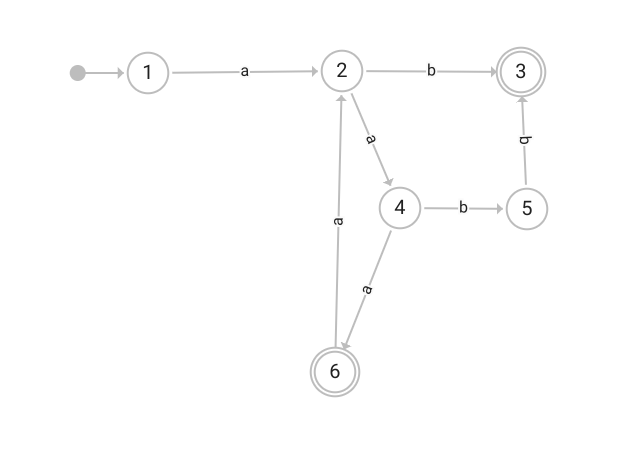
\includegraphics[width=\textwidth]{automat.png}

Tj. existuje KA (v daném případě DKA), generující tento jazyk, tedy tento jazyk je regulární. 

\item[(2)]

Formálně ověříme, jestli tento jazyk má pumpující vlastnost (již víme, že by ji měl mít, jinak by teno jazyk nemohl být regulární).

Chceme ověřit, že existuje konstanta $p \in \mathbb{N}$ taková, že $\forall$ řetězec $w \in L_1$, kde pokud $|w| \geq p$, pak platí, že existuje nějaký rozklad řetězce $w = xyz$  tak, že $|y|\geq 1$ a zárověň $|xy| \leq p$ a zárověň $\forall k\in\mathbb{N}_{0}$ platí, že $xy^{k}z \in L_1$

Formálně:

$$(\exists p \geq 1)(\forall w \in L_1)[|w| \geq p \Rightarrow (\exists x, y, z \in \Sigma^{*})(w = xyz \land |xy| \leq p \land |y| \geq 1 \land (\forall k \geq 0)(xy^{k}z \in L_1))] $$

Zárověň musíme najít tuto konstantu p nejmenší.

Zkusíme pro $p = 1$:

Vezmeme řetězec $w = a$, potom existuje právě jedno rozdělení $w$: 

\begin{align*}
& x = \epsilon \\
& y = a \\
& z = \epsilon \\
\end{align*}

Potom ale pro $k = 0$ dostaneme $xy^{0}z = \epsilon a^{0} \epsilon = \epsilon \notin L_1$. Tj. už nemůžeme pro všechny řetězce delký alespoň 1 zajistit pumpující vlastnost, musíme vzít větší konstantu $p$.

Pro $p = 2$:

Jako protipříklad vezmeme řetězec $w = ab$. Má to sice dvě různá rozdělení, ale pro každé určitě nalezneme nějaké $k$,  pro které výsledný řetězec nebude z jazyka, protože nebude sedět počet symbolů $a$ a $b$.

Například:

\begin{align*}
& x = \epsilon \\
& y = a \\
& z = b \\
\end{align*}

Potom pro $k = 0$ dostaváme $xy^{0}z = \epsilon a^{0} b = b \notin L_1$. 

Pokud zvolíme to druhé zbývající rozdělení, tak zase pro $k=0$ dostaneme prázdný řetězec a ten do jazyka nepatří. 

A žádná další rozdělení nemáme, pro toto $p = 2$ nemůžeme dokázat pumpijící vlastnost jazyka.

Pro $p = 3$:

Zvolíme zase minimální řetězec délky 3: $$w = aaa$$.

Pokud zvolíme $y = aaa$, pak $\forall k \geq 1$ pumpující vlastnost platí.

Ale pro $k=0$ dostaneme prázdný řetězec, který do jazyka nepatří. Pokud zkusíme zbývající dvě rozdělení, určitě najdeme taková $k$, kde nebude sedět počet symbolů $a$ a $b$.


Pozorování: Vidíme, že pokud pumpujeme podřetězec $aaa$, tak nikdy neporušíme podmínku na počet symbolů $a$ a $b$. Tj. obecně hledáme rozdělení, kde $y = aaa$, ale zárověň nedostaneme prázdný řetězec.

Pro $p=4$:

Minimální řetězec bude $w = aabb$. Úplně analogicky pro káždé rozdělení určitě najdeme takové $k$, že výsledný řetězec nebude patřít do jazyka, a to přes porušení správného počtu symbolů $a$ a $b$.

Pro $p=5$:

Minimální řetězec bude $w = aaaab$. Všimneme si taky, že pro káždý řetězec $w \geq 5$ máme ten řetězec ve tvaru $a^{3}a^{m}b^{m\bmod 3}, \forall m \in \mathbb{N}$

Vždycky zvolíme rozdělení:

\begin{align*}
& x = \epsilon \\
& y = a^{3} \\
& z = a^{m}b^{m\bmod 3} \\
\end{align*}

A pro káždý takový řetězec v tomto tvaru a pro každé $k \in \mathbb{N}_{0}$ platí pumpující vlastnost.

Takže pro $p = 5$ platí pumpující vlastnost pro jazyk $L_1$, která je nutnou podmínkou (nikoliv postačující) pro regularitu jazyka $L_1$. Zárověň nalezená konstanta $p = 5$ je nejmenší, protože pro všechny nižší hodnoty jsme vyvrátili pumpující vlastnosti pro určité řetězce a konstanty $k$.


\hfill $\square$

\end{description}

\noindent\rule{\textwidth}{0.4pt}
\vskip 0.3cm

\noindent
(0,5 bodu) Rozhodněte, zdali je následující jazyk $L_2$ regulární, či nikoliv. Pokud jazyk není regulární, formálně toto tvrzení dokažte. Pokud jazyk regulární je, popište jej jedním z formalismů pro popis regulárních jazyků (tj. KA, RG, nebo RV). Dále pro něj nalezněte nejmenší konstantu pumping lemma $p$ (jejíž existence je pro regulární jazyky v pumping lemma zaručena) a zdůvodněte, proč je vaše konstanta správná a nejmenší.

$$L_2 = \{ 2^m 1^n 2^j : m,n,j \in \mathbb{N} \wedge m > 1 \wedge n,j \geq 1 \wedge j \neq m+n \}$$

\section*{Řešení:}

Vidíme, že počet symbolů $2$ zprava nesmí být stejný jako počet všech ostatních symbolů zleva. 

Příklad řetězců obsažených v tomto jazyku:

$$L_2 = \left\{ 2212, 22122, 2212222, 22112, ...  \right\}$$

Pozorování: minimální řetězec je $2212$.

Zatím mohli bychom mít intuici, že tento jazyk nemá pumpující vlastnost kvůli podmínce $j \neq m + n$, zkusíme tedy vyvrátit pumpující vlastnost, tj. že pro daný jazyk $L_2$ neplatí pumpující vlastnost a tedy není splněná nutná podmínka pro regularitu tohoto jazyka (tj. použijeme obměnenou implikaci v pumping lemma):

Pokud $L_2$ nemá pumpující vlastnost, potom není regulární.

Musíme tedy dokázat negaci pumpující vlastnosti:

\begin{align*}
& \neg(\exists p \geq 1)(\forall w \in L_1)[|w| \geq p \Rightarrow (\exists x, y, z \in \Sigma^{*})(w = xyz \land |xy| \leq p \land |y| \geq 1 \land (\forall k \geq 0)(xy^{k}z \in L_1))] \equiv \\
& \equiv (\forall p \geq 1)(\exists w \in L_2)[|w| \geq p \land (\forall x,y,z \in \Sigma^{*})((w = xyz \land |xy| \leq p \land |y| \geq 1) \Rightarrow (\exists k \geq 0)(xy^{k}z \notin L_2))] \\
\end{align*}

Pokud tuto negaci dokážeme, tak z toho bude plynout, že $L_2$ není regulární.

Pro důkaz neregularity budeme dokazovat neregularitu doplňku $L_2$. Důvodem je to, že může být, že důkaz pro $L_2$ povede na práci s faktoriály. Bude jednodušší vyvratit pumpující vlastnost pro doplňěk jazyka $L_2$. 

Víme z vlástností regulárních jazyků, že regulární jazyky jsou uzavřené na operaci doplňku. Tj. platí:

$$ L \text{ je regulární } \Leftrightarrow \Sigma^{*} \setminus L = \overline{L} \text{ je regulární }$$.

T.j. vyvrátíme pumpující vlastnost pro jazyk $\overline{L_2} = \Sigma^{*} \setminus L_2$.

Konkrétně vezmeme nějaký řetězec, kde platí $j = m + n$. Libovolný takový řetězec není v $L_2$, ale jistě je v $\overline{L_2}$. Například:

\begin{align*}
& w = 22^{p}12^{p+2} \\
& w = 22_{1}2_{2}...2_{p-1}2_{p}12_{1}2_{2}...2_{p+2} \\
& max~xy = 22_{1}2_{2}...2_{p-1} \\
& min~xy = 2 \\
& min~z = 2_{p}12_{1}2_{2}...2_{p+2}
\end{align*}

Potom každé možné rozložení pro takové $w$ lze představit jako:

\begin{align*}
& x = 2^r \qquad r \geq 0 \\
& y = 2^s \qquad s \geq 1 \\
& z = 2^{t}12^{p+2} \qquad t \geq 1 \\
& \text{kde zárověň platí:} \\
& r + s + t + 1 = p + 2 \Leftrightarrow r + t = p + 1 - s \\
\end{align*}


Potom vždycky při volbě $k=0$ dostaváme:

\begin{align*}
& xy^{0}z = 2^{r}(2^{s})^{0}2^{t}12^{p+2} = 2^{r}2^{t}12^{p+2}, \\
& \text{aby tento řetězec byl z jazyka $\overline{L_2}$, musí platit:} \\
& r + t + 1 = p + 2 \Rightarrow p + 1 - s + 1 = p + 2 \Rightarrow s = 0, \\
& \text{což je spor s tím, že $s \geq 1$}
\end{align*}

To znamená, že pří žádném rozkladu pro $k = 0$ nikdy nebude výsledný řetězec z jazyka $\overline{L_2}$. Tj. neplatí pro tento jazyk pumpující vlastnost, a tím padem tento jazyk není regulární, a tím pádem není regulární i jazyk $L_2$!

\hfill $\square$

\end{document}